\fancychapter{User studies}
\label{chapter:results}

In order to evaluate the created social robot on the game playing scenario of \emph{Sueca}, a user study was conducted.
The main idea was to set up the environment in which this robot is supposed to interact with human players, and collect, in an adequate way, their feelings and perceptions.
The targeting measures are the trust on the partner, the affect felt, and also the perception of the team player's social presence.
Therefore, participants answered a questionnaire before playing with \ac{emys} and another one after the game.
The current chapter starts with the samples description and proceeds with analyses on three mentioned measures.


\section{Samples Description}
\label{sec:samples}
A group of 60 participants were included in this study with a mean age of 24,31 $\pm$ 3,852.
Out of the 60 subjects, 40 played the game with a human partner and 20 played with \ac{emys} as their team player.
These distributions aimed to collect a valid number of answers from \ac{emys} partners.
Additionally, out of the 59 subjects that revealed their gender, 20 were females and 39 were males.
Furthermore, most participants affirmed to know their partners in spite of not having played with them before, and their \emph{Sueca} knowledge was nearly medium.

\section{Trust}
\label{sec:trust}
The trust in the partner was measured by the answers of each individual, before and after the game session, to the Human-Robot Trust Questionnaire \cite{Schaefer2013}.
Consequently, the following three questions arose:
\begin{itemize}
\item Are there changes in trust after the experience of interacting with the \emph{Sueca} partner?
\item Are the trust levels influenced by the partner (robot or human)?
\item Are the trust levels influenced by the game results?
\end{itemize}


\subsection*{Are there changes in trust after the experience of interacting with the \emph{Sueca} partner?}
The statistical test used to infer a conclusion about this question was a Mixed ANOVA, with time as a factor of 2 levels and condition (partner) as the between-subjects factor.
Additionally, assumptions were tested to guarantee the data validity.
The dependent variable (time) showed a significant effect with p = 0.03.
However, by adding the independent variable (condition), the effect was not significant with p = 0.65.

\begin{figure}[h!]
  \centering
    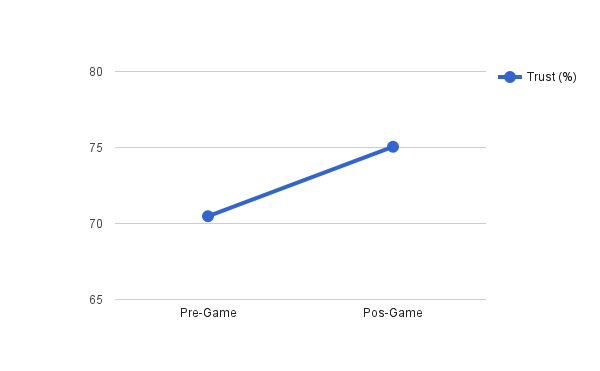
\includegraphics[width=0.7\textwidth]{./img/6/trustMixedANOVA}
  \caption{Evolution of the trust percentage between the two time levels}
\label{fig:trustMixedANOVA}
\end{figure}

Figure~\ref{fig:trustMixedANOVA} presents the evolution of the trust percentage between the two time levels, before the game and after the game.
The trust values correspond to estimated means separated by time, since it was the only significant variable.

\textbf{Answer:} There were significant differences in Trust before and after playing \emph{Sueca}, but there was not significant differences between \emph{Sueca} partners at different time levels.



\subsection*{Are the trust levels influenced by the partner (robot or human)?}
The statistical test used to infer a conclusion about this question was the Welch Test, with condition as factor and pos-game trust as dependent variable.
As a result, the condition effect was proved with p = 0, suggesting the means of trust were significantly different between having a robot partner or a human partner.

\textbf{Answer:} There were significant differences in Trust between different \emph{Sueca} partners.


\subsection*{Are the trust levels influenced by the game results?}
The statistical test used to infer a conclusion about this question was the Two-Way ANOVA, with condition and game result as factors and pos-game trust as dependent variable.
The effect of condition was significant, with p = 0.01 (already proved in the previous question).
On the other hand, the game result cannot reject the null hypothesis with p = 0.065, and therefore proves an insignificant effect on the trust measure.
Moreover, the effect of both condition and game result also proved to be insignificant with p = 0.507.

\textbf{Answer:} There were not significant differences in Trust between different game results.


\section{Social Presence}
\label{sec:socialPresence}
Each subject answered the Networked Minds Questionnaire after playing the game in order to measure the social presence of his partner \cite{Harms2004}.
This measure of social presence includes six different subcategories: co-presence, attentional allocation, perceived message understanding, perceived affective understanding, perceived emotional interdependence, and perceived behavioural interdependence.

By considering this measure in a \emph{Sueca} scenario, one question arose:
\begin{itemize}
\item Is the social presence influenced by the partner (robot or human)?
\end{itemize}

\subsection*{Is the social presence influenced by the partner (robot or human)?}
The statistical test used to infer a conclusion about this question was the One-Way ANOVA, with condition as factor and each social presence subcategories' values as dependent variable.
The condition presented the following statistical effects of each subdimension results:
\begin{itemize}
\item There was not a statistically significant difference between the co-presence as determined by one-way ANOVA (F = 1.559, p = 0.217);
\item There was not a statistically significant difference between the attentional allocation as determined by one-way ANOVA (F = 0.002, p = 0.965);
\item There was a statistically significant difference between the perceived message understanding as determined by one-way ANOVA (F = 0.081, p = 0.777);
\item There was a statistically significant difference between the perceived affective understanding as determined by one-way ANOVA (F = 7.850, p = 0.007);
\item There was a statistically significant difference between the perceived affective interdependence as determined by one-way ANOVA (F = 4.148, p = 0.046);
\item There was not a statistically significant difference between the perceived behavioural interdependence as determined by one-way ANOVA (F = 0.699, p = 0.406).
\end{itemize}

The social presence of partner evidenced discrepancies for the two conditions in two subdimensions: perceived affective understanding and perceived emotional interdependence.
As a result, Figure~\ref{fig:perceiveEmoAff} shows theses discrepancies.

\begin{figure}[h!]
  \centering
    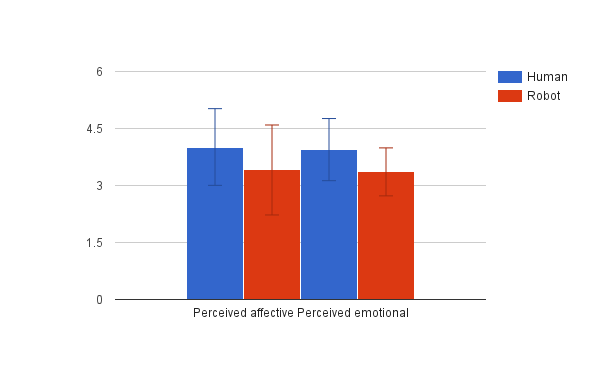
\includegraphics[width=0.7\textwidth]{./img/6/perceiveEmoAff}
  \caption{Perceived affective understanding and perceived emotional interdependence means for each  condition}
\label{fig:perceiveEmoAff}
\end{figure}

\textbf{Answer:} There were not significant differences in Social Presence between \emph{Sueca} partners.


\section{Affect}
\label{sec:affect}
The affect was measured by the answers of each individual, before and after the game session, to the PANAS Questionnaire.
It is divided into positive and negative affect and, therefore, there are two questions to answer:
\begin{itemize}
\item Are there changes in the positive affect after the experience of interacting with the \emph{Sueca} partner?
\item Are there changes in the negative affect after the experience of interacting with the \emph{Sueca} partner?
\end{itemize}

\subsection*{Are there changes in the positive affect after the experience of interacting with the \emph{Sueca} partner?}
In order to answer this questions, a Mixed ANOVA has been run on the collected data, with time as a factor of 2 levels and condition as the between-subjects factor.
So, time proved to have a statistical significant effect on the positive affect, p = 0.008.
On the other hand, the time levels by condition did not present a significant effect on the positive affect, p = 0.488.

\begin{figure}[h!]
  \centering
    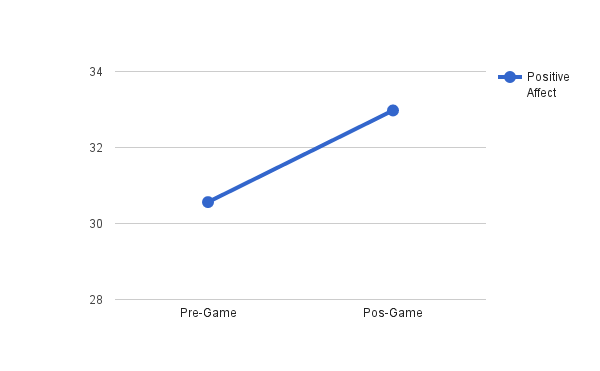
\includegraphics[width=0.7\textwidth]{./img/6/positiveAffect}
  \caption{Evolution of the positive affect between the two time levels}
\label{fig:positiveAffect}
\end{figure}

Figure~\ref{fig:positiveAffect} evidences the evolution of the positive affect before and after playing \emph{Sueca} with \ac{emys}.

\textbf{Answer:} There were significant differences in Positive Affect before and after playing \emph{Sueca}, but there was not significant differences between \emph{Sueca} partners at different time levels.

\subsection*{Are there changes in the negative affect after the experience of interacting with the \emph{Sueca} partner?}

\clearpage
